\documentclass[12pt]{article}

% ----------------------------------------------------------------------
% Define external packages, language, margins, fonts, new commands 
% and colors
% ----------------------------------------------------------------------
\usepackage[utf8]{inputenc} % Codification
\usepackage[english]{babel} % Writing idiom
\usepackage{multirow}
\usepackage[export]{adjustbox} % Align images
\usepackage{amsmath} % Extra commands for math mode
\usepackage{amssymb} % Mathematical symbols
\usepackage{anysize} % Personalize margins
    \marginsize{2cm}{2cm}{2cm}{2cm} % {left}{right}{above}{below}
\usepackage{appendix} % Appendices
\usepackage{cancel} % Expression cancellation
\usepackage{caption} % Captions
    \captionsetup{labelfont={bf}}
\usepackage{cite} % Citations, like [1 - 3]
\usepackage{color} % Text coloring
\usepackage{fancyvrb}
\usepackage{fancyhdr} % Head note and footnote
    \pagestyle{fancy}
    \fancyhf{}
    %\fancyhead[L]{\footnotesize Graduating } % Left of Head note
    \fancyhead[R]{\footnotesize UNYT} % Right of Head note
    \fancyfoot[L]{\footnotesize Graduating Project} % Left of Footnote
    \fancyfoot[C]{\thepage} % Center of Footnote
    \fancyfoot[R]{\footnotesize Department of Computer Science} % Right of Footnote
    \renewcommand{\footrulewidth}{0.4pt} % Footnote rule
\usepackage{float} % Utilization of [H] in figures
\usepackage{graphicx} % Figures in LaTeX
\usepackage[colorlinks = true, plainpages = true, linkcolor = istblue, urlcolor = istblue, citecolor = istblue, anchorcolor = istblue]{hyperref}
\usepackage{indentfirst} % First paragraph
\usepackage[super]{nth} % Superscripts
\usepackage{siunitx} % SI units
\usepackage{subcaption} % Subfigures
\usepackage{titlesec} % Font
    \titleformat{\section}{\Large\bfseries}{\thesection}{1em}{}
    \titleformat{\subsection}{\large\bfseries}{\thesubsection}{1em}{}
    \titleformat{\subsubsection}{\normalsize\bfseries}{\thesubsubsection}{1em}{}
    \fancyfoot[C]{\thepage}
% Random text (not needed)
\usepackage{duckuments}
\usepackage{booktabs}
\usepackage{url}
\usepackage{graphicx}

% New and re-newcommands
\newcommand{\HRule}{\rule{\linewidth}{0.5mm}} % Specific rule definition
\renewcommand{\appendixpagename}{\LARGE Appendices}
\newcommand{\sectiononlytoc}[1]{%
    \par
    \refstepcounter{section}%
    % Don't print sectional unit; just add to ToC and update the Left header
    \addcontentsline{toc}{section}{\protect\numberline{\thesection}#1}%
    %\fancyhead[L]{#1}% Add chapter title in Left header
}

% Colors
\definecolor{istblue}{RGB}{3, 171, 230}
\definecolor{dkgreen}{rgb}{0,0.6,0}
\definecolor{gray}{rgb}{0.5,0.5,0.5}

%%%%%%%%%%%%%%%%%%%%%%%%%%%%%%%%%%%%%%%%%%%%%%%%%%%%%%%%%%%%%%%%%%%%%%%%
%                                 Document                             %
%%%%%%%%%%%%%%%%%%%%%%%%%%%%%%%%%%%%%%%%%%%%%%%%%%%%%%%%%%%%%%%%%%%%%%%%
\begin{document}

% ----------------------------------------------------------------------
% Cover
% ----------------------------------------------------------------------
\begin{center}
    \mbox{}\\[2.0cm]
    \LARGE Enabling Multilingual Communication: Automated Lip-synchronization Dubbing for Albanian Videos
\end{center}

\vspace{10cm}

\begin{center}
    \Large ALDO DIKU
\end{center}

\vspace{5cm}

\begin{center}
    \Large UNIVERSITY OF NEW YORK TIRANA
\end{center}
\begin{center}
    \large \Large JULY 2025
\end{center}
\thispagestyle{empty}

\setcounter{page}{0}

\newpage
% ----------------------------------------------------------------------
% APPROVAL PAGE
% ----------------------------------------------------------------------
\noindent This is to certify that I have read this project and that, in my opinion, it is fully adequate, in scope and quality, as a thesis for the degree of Bachelor of Arts in Computer Science.

\vspace{4cm}

\noindent
(Title and Name) \hspace{4cm} \\
(Project Advisor) \hspace{2cm} \underline{\hspace{2cm}} \hspace{1cm} \underline{\hspace{8cm}}

\vspace{3cm}

\noindent This is to confirm that this thesis complies with all the standards set by the Department of Computer Science of University of New York Tirana.

\vspace{2cm}

\noindent Date: \hspace{5cm} \hfill Seal/Signature: \hspace{5cm}

\setcounter{page}{1}

\newpage

% ----------------------------------------------------------------------
% PLAGARIZM CLEARANCE PAGE
% ----------------------------------------------------------------------
\noindent I hereby declare that all information in this document has been obtained and presented in accordance with academic rules and ethical conduct. I also declare that, as required by these rules and conduct, I have fully cited and referenced all material and results that are not original to this work.

\vspace{2cm}

\noindent \hspace{7.5cm} First Name, Last Name:\\
\\
\vspace{1.0cm}
\noindent \hspace{7.3cm} \text{Signature:} % NO CLUE WHY THIS IS 7.3 AND NOT 7.5 LIKE ABOVE

\setcounter{page}{2}

\newpage

% ----------------------------------------------------------------------
% ABSTRACT
% ----------------------------------------------------------------------
\sectiononlytoc{Abstract}
\begin{center}
    
    \vspace{0.5cm}
    
    ABSTRACT
    
    \vspace{1cm}
    
    \centering{ ENABLING MULTILINGUAL COMMUNICATION: AUTOMATED LIP-SYNCHRONIZATION DUBBING FOR ALBANIAN VIDEOS}
    
    \vspace{1cm}
    
    Diku, Aldo.
    
    BA. in Computer Science
    
    Thesis Advisor: Prof. Miralda Çuka
    
    June 2025, 20 pages
    
    \vspace{1cm}
\end{center}

\noindent Using available methods and tools (which i will mention when i gather all the tools and methods) to create lip-synced dubbed videos from an albanian video input and outputting a video of the same speaker in another language with the lips moving according to that languages movements. 
    
\vspace{1cm}
    
\noindent Keywords: Lip-sync, dubbing, albanian language

\newpage

% ----------------------------------------------------------------------
% Acknowledgements
% ----------------------------------------------------------------------

\sectiononlytoc{Acknowledgements}

First and foremost, I would like to express my sincere gratitude to my advisor, Professor Miralda Çuka, for their invaluable guidance, unwavering support, and insightful feedback throughout this project. Their expertise and encouragement were instrumental in shaping this work.

Finally, I am grateful for the support of my family and friends. Something something a little bit longer and better made.

\newpage


% ----------------------------------------------------------------------
% Contents
% ----------------------------------------------------------------------
\tableofcontents 

\newpage

% ----------------------------------------------------------------------
% Body
% ----------------------------------------------------------------------
\section{Introduction}
\subsection{Background of the study}
The increasing globalisation of online content consumption presents a significant challange for video creators aiming to reach diverse audiences, thereby creating the need to produce multilingual versions of their work. Being able to make only one video and have it transform into multiple languages will help creators but also the target audience as well. Cutting down on the time and money it takes to make two or more videos with the same subject but in different languages. One such case is a youtube creator named der8auer from Germany, for the same topic he creates two videos, one in english and one in german. Sometimes his videos are quite long and having to do them again in another language will tire you out. Having a model that can take your video, translate it into another language and synchronize your lips to the movement of the language of your choosing would be a tool in your arsenal. Some of the usages of this lip-sync dubbing technology are: video dubbing and translation, real-time Face-to-Face translation that will be possible in the future and multilingual communication, gaming and virtual environments reduced cost and labor and time in this case, entertainment and content creation, speech recognition and lip-reading. Film, entertainment and media production. Education and training videos, especially in cases where there is a diverse workforce. It also has promissing applications in areas for speech therapy, language learning and assistive communication devices for individuals with hearing impairments \cite{biomedinformatics4010023}. Advancments in Machine Learning (ML) have made it possible to have Automatic Speech Recognition (ASR) 

\subsection{How lip synchronization works}
Phonemes are the distinct units of sound in speech, and visemes are visual representations of phonemes. Think phonemes as the audio and visemes as the video. Visemes serve to map sounds (phonemes) to corresponding mouth positions or shapes. The goal is to go from the audible  to the visual (visemes). Visemes group similar-looking mouth shapes, which reduces the complexity required for animation. Relating the extracted audio features to the corresponding visual mouth shapes and facial expression. Mapping phonemes down to a smaller number of visemes gives artists fewer expressions to pose. The history of lip-syncing comes from animation and in particular two-dimentional cartoons where artists had to make facial movement according to the sounds of speech \cite{game-lipsynch}. Lip-synchronization is a field that has been studied since 1994 \cite{earliest-lip-synch}, where Automatic lip-sync (ALS) could be used for animating cartoons realistically making the mouth movement more smoother and have it a more natural feel and could also help in aiding people with hearing disability. Later in 1997 a new method was proposed where they used Fast Fourier Transform (FFT) for speech signal analysis, statistical measures called "moments" are used to describe the shape of the FFT. Mouth parameter measurements are used to measure the jaw position, the height of the maximum vertical opening between the lips and horizontal opening of the lips. This method did not require phonemic analysis or prior knowledge of the speech content. ObamaNet was an innovative architecture released in 2017, it used a time-delayed Long Short-Term Memory (LSTM) network to produce synchronized lip-synch videos. The network learned to map raw audio feature to corresponding mouth shapes based on hours of high-quality videos of a specific target person \cite{ObamaNet}. Convoluted Neural Networks (CNN) played an important role in lip-synchronization as it helped in feature extraction for visual features, and image processing and generation. CNNs are often used with other models like LSTM blocks, or encoder and discriminator networks based on a Generative Adversarial Network (GAN). A study by Pawar et al. (2024) focused on Marathi, an Indian language which has a shortage of datasets, similar to that of the Albanian language \cite{PAWAR2024100084}. Integrating CNNs with adversarial training and including RNN-based architectures, specifically LSTM for lip-synch generation, Song et al. (2019), Sadoughi et al. (2021) and Li et al (2021) also used a combination of CNN, RNN, GANs and LSTMs \cite{Audio-driven-facial-animation} \cite{Li_2021}. Another similar study by Exarchos et al. (2024) for lip-reading in Greek language tackeled the scarcity of datasets available. The study proposed a combination of 3D CNNs and LSTM networks for word recognition from lip movements.  

\subsection{Methodology}
A key limmitation encountered was the lack of suitable Albanian video datasets, specifically open-license content with direct-to-camera speech, reflecting the broader challange of working with low-resource languages in multimedia applications. To address the first issue, custom video contennt was created featuring self-recorded footage in a one by one aspect ratio and lowest camera setting to save. The first step for this project was the data creation, seeing as there is not a lot of free and publicly available free-use content I can use we had to create the data myself.
Videos were recorded at 1440x1440 resolution (1:1 aspect ratio) at 30 frames per second, with durations ranging from 10 seconds up till 5 minutes. The study at (citation needed for the optimal length of time of the videos) found that the optimal length time was for videos with one word in them. To adapt to this, a script was made to create small chunks of videos to be closer to that optimal format. Videos could have been created by following and reading a script thereby avoiding the transcipiton step, however we want to create a workflow that will take any video of an albanian speaker and turn it into a dub lip synched video.

\begin{figure}[h!]
    \centering
    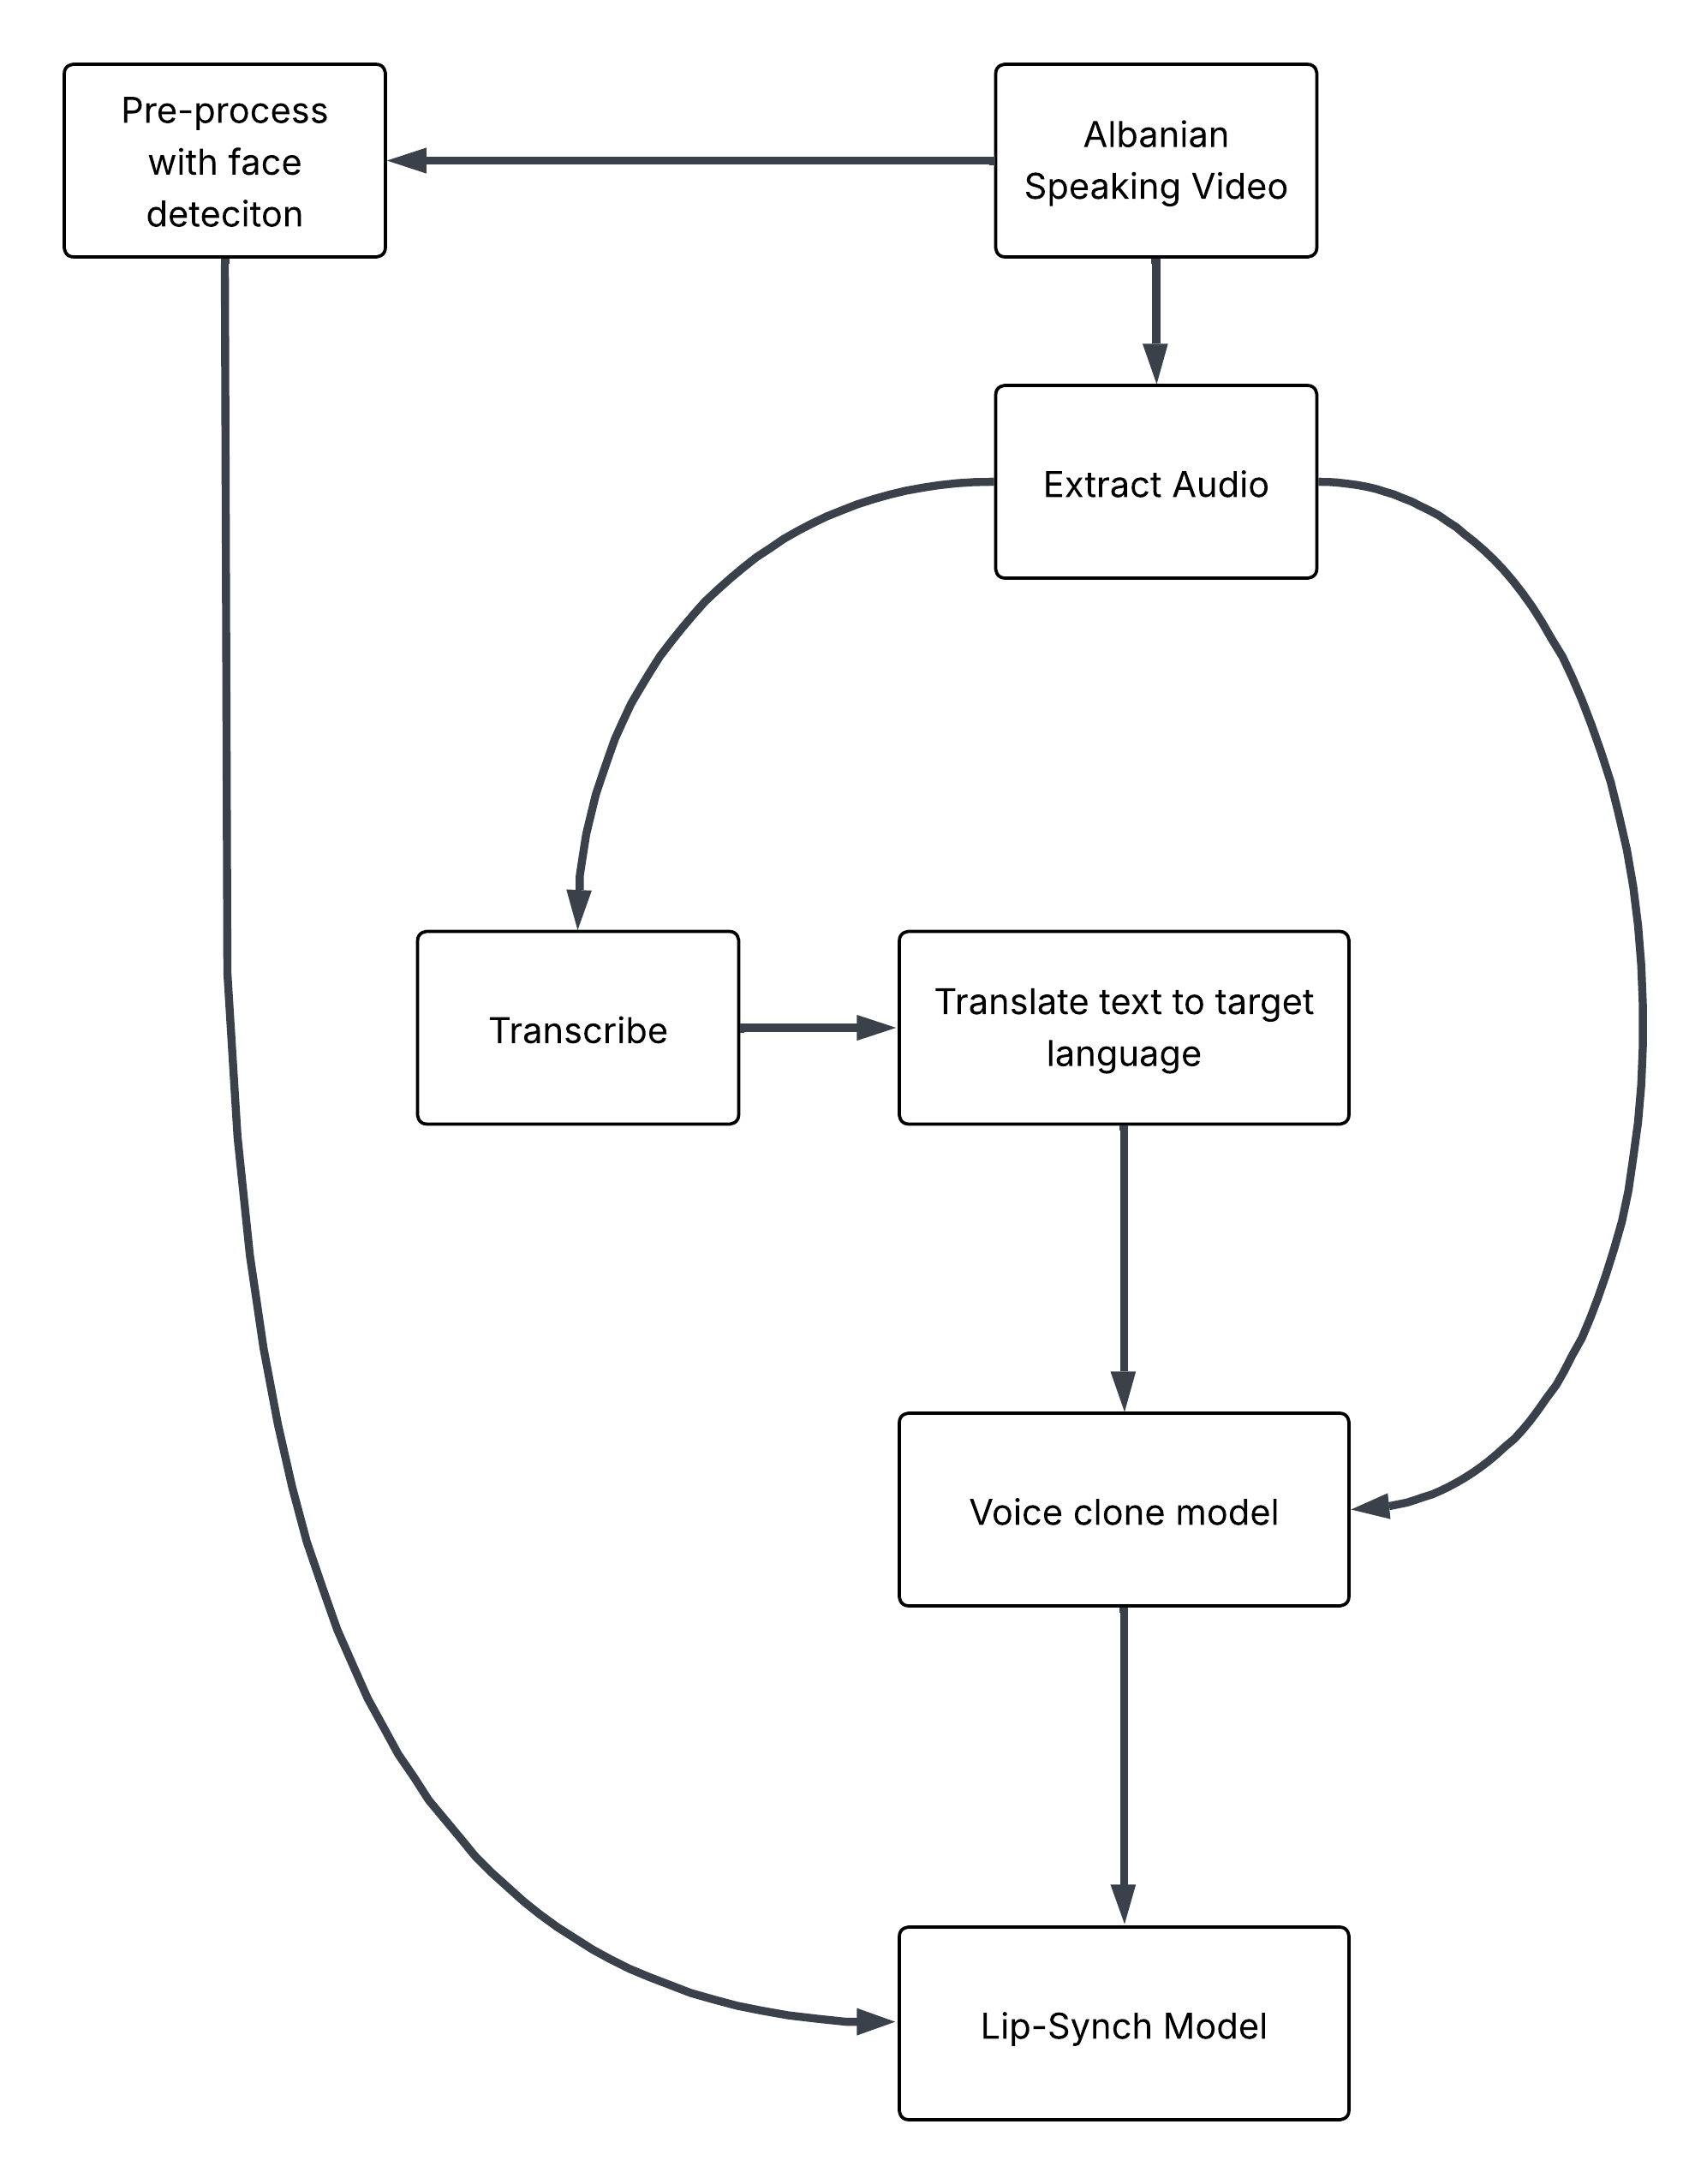
\includegraphics[width=0.5\textwidth]{images/work-flow.png}
    \caption{Work Flow}
    \label{fig:work-flow}
\end{figure}

Audio was then extracted from the videos using ffmpeg package, Pulse Code Modulation, Signed 16-bit, Little Endian (pcm\_s16le), a lossless, uncompressed audio codec format, 16000hz sample rate and monophonic, meaning single audio channel.  which will be used for transcription and for the base of the voice cloning tool before inputing it into the final lip synchronization model. For the audio extraction ffmpeg library was used, and audio was extracted in a lossless codec, 16000hz sample rate and signed 16-bit Pulse Code Modulation (PCM), per Google Speech-to-text API documentation \cite{google_api_docs}.\\
The audio gets sent through an Automatic Speech Recognition model, converting spoken language into written text. and gets saved in a text file, each line contains the name of the file transcripted and a colon separates it from the text. After several tests of three models, Google Speech to Text Chirp 2, Kushtrims and Neura, the latter one was selected as being the most accurate \cite{google_api_docs}\cite{kushtrim}\cite{neura}.\\
Transcripted text is translated to a target language that is supported by the voice cloning model. Using deep-translator python package and utilizing google translate as its core. Audio of the same file is used as reference to make a voice clone using OpenVoice, in the target language, a check is made if the cloned output is longer or shorter than the reference audio\cite{openvoice}. Another clone is made with the speed of the audio modified to be as close as possible to the original. OpenVoice offers emotion and accent cloning offering flexible voice control. The translated text will be used as the base of what the voice clone should output. OpenVoices Zero-shot cross-lingual voice cloning can generate speech that can be not present in the multi-lingual training dataset used by the model. There is "native" support and generalisation of voice clones. The native support is offered for languages like english, spanish, french, chinese, japanese and korean in the second version of OpenVoice.\\
The reference video is processed to be cropped in a 512x512, 25 frames per second format with the face centered, this was made using a face detection model which would detect faces in every frame of the video, from there we take the center and crop accordingly. Googles mediapipe framwork was used for the face detection task \cite{GoogleFaceDetector}. This format is a pre-requisite before inputting videos into the final lip-synching model.  Pre-emptive tests were done on the videos to see if the face detector worked as intended and could detect a face in every frame of the videos. 

After translating, the translated text and the original audio are used to make the voice clone. We need the original audio of the transcript because of emotions displayed in the audio can be used by the voice cloning tool.\\
Cloned voice and the original video from where the cloned voice was based on are then used to train the lip synchronization model. 

\textbf{One of the challanges of creating a lip synchronization in videos is the need for the lip movements to accurately align with a specified target speech segment, especially in multilingual and unconstrained environment. Visual data falling out of sunc with updated audio and inaccurate lip movements in target videos.}\\
CNN and Generative Adversial Networks (GANs) to create the lip movements that sync up, this combined with a Discriminator Network which would try and detect the GANs fake lip movements and real ones, pushing each other to get better.

\subsection{Work Steps Overview}

From the video we need to get the transcription in albanian, for this step several models were tried and tested although only the google cloud API were the best performing one. The next and easiest step to implement is translating the transcription to the target language, translation has come a long way and there are many tools which can achieve high accuracy, we decided to use googe translate. The following task is to take the translated transcript and use a voice cloning tool/model to make the voice dubbing. \textbf{There are several models availabe which have not been tested by me yet.} After this we have to use object tracking to track the mouth area in the video to then use the deep learning model for lip frame creation. \textbf{This depends heavily on the model the will be applied.}

\subsection{Audio transcription}
The first step of the project is extracting audio from the videos and this was done using the open-source ffmpeg package. Going by the suggestions for optimizing transcription quality through googles speech-to-text API documentation \cite{google_api_docs}, best practices, the audio was sampled at 16000 Hz, converted into a singned-integer bitrate, and in a lossless pcm\_s16le format. One group of audio files were made in a lossless format, signed 16bit PCM (linear16), 16000hz sampling rate. While the other folder, was made with the same codec but with 48000hz sampling rate.\\There is no open-source ASR model for Albanian language, and the amount of Albanian audio dataset is very low. Florijan (2023) managed to collect 40 hours of diverse accents, dialects and speech styles of Albanian audio, the purpose was to exceed an initial accuracy target of 45\% \cite{florijan-qosja}. This data was filtered out of 133 hours available, going through validation accuracy above 0.9 used for training. The base model used for this was Deep Speech 2 by Baidou \cite{deep-speech}, consisting of a combination of CNNs and RNNs. The model did managed to reach an accuracy of 46.3\%, passing the threshhold but the model is not suitable for real world application. To test if there was another better model suitable for the dataset used by Florijan we used the Whisper model by OpenAI \cite{openai_whisper}. At first we tested the biggest model out of the box to check its performance, There are seven distinct whisper models whos difference lies in the parameter size and support for english only. Whisper is trained on 680,000 hours of labeled audio data, 438,218 hours of English language only, 117,000 hours covering 96 languages, Albanian included, though it does not mention the amount of hours for each language. Audio was sampled at 16000hz in mono, similar to that of Googles documentation. Its English ASR performance was very close to that of a human. Models range from tiny (39 million parameters) to large-v3 (1550 million parameters) these models were tested, attempts to fine-tune the large-v3 model with the dataset from Florijan we fruitless as the training time for such large parameter model was over 177 hours on a RTX 3080Ti 12GB Nvidia graphics card and 32GB of RAM. All models were tested from ones with the biggest parameter to the smallest, the only model that we could feasibly train was the whisper-small with a little bit more than 8 hours. ASR systems are evaluated using a Word Error Rate (WER) score, measuring the number of errors (substitutions, insertions and deletions) needed to transform the output of the ASR system into the reference transcript or ground truth. A lower WER score indicates a better performance in \ref{eq:WER} we can see the formula used for the calculation. The fine-tuned whisper-small model achieved a 61.52\% WER, not usable in any application. Testing the accuracy of the whisper-large-v2 model as a baseline reference without any fine-tuning resultet in a 55.1\% Word Error Rate (WER) accuracy, the larger whisper-large-v3 model did not have much change and managed to score a 49.45\% WER, both of these not up to par. Facebooks Wav2Vec2 baseline model with 960 hours of training data was tested and managed to achieve a 97.74\% WER \cite{facebook-wav2vec}. 

\begin{equation}
\label{eq:WER}
WER = \frac{S + D + I}{N} = \frac{S + D + I}{S + D + C}
\end{equation}

Where:
\begin{itemize}
    \item S is the amount of substitutions,
    \item D is the amount of deletions,
    \item I is the amount of insertions,
    \item C is the amount of correct words,
    \item N is the amount of correct words.
\end{itemize}

From this point onward the search continued into closed systems, offered comercially. Googles Speech to Text API offered support for Albanian language and had free credits for first time user. Their system gives a confidence score for each transcription section and confidence score in individual words aswell. After transcription, a subtitle file format was also available to check the timings of when each word or sentence is spoken, this is an increadibly usefull feature as we could use it to cut the videos into smaller chunks as Pawar et al. (2024) experienced accelerated training process and improved performance when utilising a "vVISWA" dataset composed of isolated words \cite{PAWAR2024100084}. In the first test Googles Speech to Text API, using Chirp 2 as a model, managed to achieve a WER score of 10.7\%. Kushtrims model based on the whisper-large-v3-turbo and fine-tuned with 200 hours of curated Albanian audio with diverse dialect, hosted on the Hugginface Spaces, the model weights were not opensource, nor was the dataset used for the training \cite{kushtrim}. It did not offer a confidence score nor a SRT file with audio timings.The model could be accessed for inference using the API available from Gradio, which is how the transcriptions were processed, however the model was quite slow in times as more than one individual would try to transcribe audio at the same time, increasing the transcription time a lot, in some cases taking more than three hours for twelve seconds of audio. At a later point the model was updated with an additional 100 hours of Albanian audio. Both versions of the model were evaluated, in table \ref{tab:firs_test} we can see the scores for all models, and Kushtrims managed to get a 16.46\% WER. The other ASR model tested was Neuras \cite{neura}, a comercially available product, we were granted access and free credits. Their website advertises the model as having a 93\% accuracy, which a bit of an underestimation on their part as it scored a 3.09\% WER which is equivalent to 96.91\% accuracy. The first set of audio files contained casual speech and did not have language that would be deemed difficult to understand or hear, testing was done for ten files, comparing the ground truth to the hypothesis file.\\
WER as a metric has its limmitations, from the formula we can see that the substitutions, deletions and insertions have the same weight. A minor misspelling might have the same weight as a word that completly changes the meaning of the sentence. It also doesnt take in consideration a mistake in letters inside a word. For example, the word "duket" was incorrectly transcribed as "duhet", in this case the whole word is a mistake. All unneccessary elements are removed, punctuation, making numbers into 123. The core of the WER calculation is finding the minimum number of edits needed to transform the hypothesis (transcription) text into the reference (ground truth) text. This is typically done using a dynamic programming algorithm, specifically the Levenshtein distance algorithm, applied at the word level.
\begin{table}[h!]
\centering
\caption{Error Analysis for Challenging Albanian Scripts}
\label{tab:firs_test}
\begin{tabular}{lccc|ccc|ccc}
\toprule
\textbf{File ID} & \multicolumn{3}{c}{\textbf{Neura}} & \multicolumn{3}{c}{\textbf{Kushtrim}} & \multicolumn{3}{c}{\textbf{Google API}} \\
\cmidrule(lr){2-4} \cmidrule(lr){5-7} \cmidrule(lr){8-10}
 & \textbf{S} & \textbf{D} & \textbf{I} & \textbf{S} & \textbf{D} & \textbf{I} & \textbf{S} & \textbf{D} & \textbf{I} \\
\midrule
File 1 & 0 & 0 & 0 & 2 & 0 & 0 & 1 & 0 & 0 \\
File 2 & 0 & 0 & 0 & 8 & 0 & 0 & 7 & 0 & 0 \\
File 3 & 0 & 0 & 0 & 27 & 4 & 3 & 14 & 17 & 1 \\
File 4 & 27 & 7 & 4 & 53 & 15 & 24 & 25 & 7 & 3 \\
File 5 & 2 & 0 & 1 & 31 & 3 & 7 & 18 & 7 & 6 \\
File 6 & 0 & 0 & 0 & 6 & 0 & 0 & 2 & 0 & 0 \\
File 7 & 0 & 0 & 0 & 12 & 2 & 6 & 13 & 2 & 6 \\
File 8 & 0 & 0 & 0 & 6 & 0 & 1 & 4 & 0 & 0 \\
File 9 & 2 & 0 & 0 & 12 & 0 & 3 & 11 & 0 & 5 \\
File 10 & 2 & 0 & 0 & 10 & 3 & 2 & 5 & 2 & 0 \\
\midrule
\textbf{Total Errors} & \textbf{33} & \textbf{7} & \textbf{5} & \textbf{167} & \textbf{27} & \textbf{46} & \textbf{100} & \textbf{35} & \textbf{21} \\
\textbf{Overall WER} & \multicolumn{3}{c}{\textbf{3.09\%}} & \multicolumn{3}{c}{\textbf{16.46\%}} & \multicolumn{3}{c}{\textbf{10.70\%}} \\
\bottomrule
\end{tabular}
\end{table}

A second test was made reading along a script made with the purpose of being a difficult dialog. Five new videos were created, audio extracted and we tested Googles Chirp 2, Kushtrims and Neuras model as having the best results for a further analysis. Table \ref{tab:wer_hard} shows the results from the tested audio, very different results shown from the first test, Neuras accuracy dropped close to their advertised numbers, Kushtrims model was the one that moved less, although we have to keep in mind that this was the model with 300+ hours of training data, dispite this the models performance decreased. An anomaly was detected with Kushtrims model output because the number of Insertions is 52, in the transcription there were added words "Piii" after the end of the audio file which was not present in the other models. Removing these anomalies the models performance improves to 13.01\%, the number of insertions dropped from 52 to 30. Googles Chirp 2 had the best results, achieving a 5.17\% WER score, this could be the result of having a larger and more diverse dataset compared to Neuras model which might have more audio content with everyday speech rather than scienfic language.
\begin{table}[h!]
\centering
\caption{Second Analysis WER score}
\label{tab:wer_hard}
\begin{tabular}{lccc|ccc|ccc}
\toprule
\textbf{File ID} & \multicolumn{3}{c}{\textbf{Neura}} & \multicolumn{3}{c}{\textbf{Kushtrim}} & \multicolumn{3}{c}{\textbf{Google API}} \\
\cmidrule(lr){2-4} \cmidrule(lr){5-7} \cmidrule(lr){8-10}
 & \textbf{S} & \textbf{D} & \textbf{I} & \textbf{S} & \textbf{D} & \textbf{I} & \textbf{S} & \textbf{D} & \textbf{I} \\
\midrule
File 1 & 3 & 0 & 1 & 4 & 0 & 0 & 4 & 0 & 0 \\
File 2 & 8 & 0 & 1 & 4 & 0 & 0 & 4 & 0 & 0 \\
File 3 & 5 & 0 & 0 & 6 & 2 & 52 & 2 & 17 & 1 \\
File 4 & 5 & 1 & 1 & 4 & 1 & 1 & 5 & 1 & 1 \\
File 5 & 5 & 0 & 1 & 6 & 0 & 1 & 2 & 0 & 2 \\
\midrule
\textbf{Total Errors} & \textbf{26} & \textbf{1} & \textbf{4} & \textbf{24} & \textbf{3} & \textbf{54} & \textbf{21} & \textbf{1} & \textbf{3} \\
\textbf{Overall WER} & \multicolumn{3}{c}{\textbf{7.08\%}} & \multicolumn{3}{c}{\textbf{18.49\%}} & \multicolumn{3}{c}{\textbf{5.17\%}} \\
\bottomrule
\end{tabular}
\end{table}

Implementation of Googles API was the most challanging of the three models, as there were many different configurations, and the results varied when accessing it through the API. While Google's web UI offered more consistent transcriptions, the process required manual effort. Having the better accuracy of all tested models on the majority of the dataset and because of the nature of the audio content of the dataset being conversational language, Neura was chosen as the transcription model to go forward with the project. \textbf{Later tests on Kushtrim model show a lot of errors, repetions of words. Not sure if it should be included.}

\subsection{Voice Cloning}
\textbf{Should add a bit of history for the voice cloning, different models, architectures, its uses etc.}\\Voice cloning is a subtask of speech synthesis, using deep learning to create speech imitating a specific voice. Prioritizing the preservation of the identity of the target speaker. Modern systems use a combination of speaker embedder (or encoder) to capture unique voice characteristics, a synthesizer to predict acoustic representations from text and the speaker embedding, and a cocoder to convert these representations into speech.\\
The NAUTILUS system from \cite{NAUTILUS} has the ability to clone untranscribed speech, using a small amount of untranscribed speech, cited as about five minutes. Experiments coparing performance with different amounts of adaptation data show that Mean Opinion Score (MOS) for naturalness and similarity can improve significantly from five seconds to 15 seconds of untranscribed audio, plateauing or showing only minor improvement beyond that (e.g. 30 or 60 seconds)\cite{Unified_system_for_Voice_Cloning_and_Voice_Conversion}.\\ 
Noisy audio can negatively impact the quality of generated speech, a real-time voice cloning system notes that generated speech can have low intelligibility due to artifacts, such as murmurs, hums, or noisy audio \cite{Real-time_voice_cloning_system}.\\
Because of different trainning and test datasets and metrics used, MOS for example is a subjective measurement.
A paper in 5th of May 2025 was released by \cite{viola-voice-role-play} which created a foundation model for realt-time autonomous interaction and voice role-play. \\
*Show differences between intra-lingual and cross-lingual models in voice-cloning research*. 

Using the translated text into the language of our choice we can then try and use a voice cloning model to make the voice dubbing. A lot of models were available for this task, Nari Labs released Dia, in 22nd April 2025, coqui-ai, which a lot of other models are based on. 


Fine-tuuning the voice cloning models since they might respond better to more of my voice.

\section{Lip synch model}
Before deep learning lip-sync was achieved using viseme-based and rule-based system, mapping phonemes to corresponding visual mouth shapes. These methods were more commonly used in cartoons as they lacked the realism and fluidity of natural speech \cite{automatic-lip-synch-methods-in-games}\cite{https://doi.org/10.1002/vis.4340020404}\cite{computers14010007}. 

\section{Future improvements}



\subsection{Questions raised}
List of questions:
\begin{itemize}
    \item How do we decide if we are going to use a transcription or not?
    \item How do we know if the transcription is correct programatically?
    \item How should the data be prepared for the lip-synchronization model?
    \item Video format, 30 frames per second or 25, quality of the video, resolution, etc.
    \item Audio format, mp3, lossless, bitrate, etc.
    \item How does the duration of video chunks used during preprocessing impact the performance of the final machine learning model, and what chunk length yields the best trade-off between information retention and computational efficiency?
    \item How are voice cloning models evaluated, as it feels like it should be done with a human evaluation and that is faulty most of the time?
    \item Which would be the best model for the lip-synchronization task based on the data we have?
    \item Best way to handle differences between original audio timing and the voice cloned sample timing. (slow down the voice? speedup)
    \item Is an LLM better than a traditional tool for translating? Neural Machine Translation (NMT) vs Large Language Models.
\end{itemize}
AS for the optimal length of the video chunks, the study done by \cite{PAWAR2024100084} faced challanges with lengthy continuous speech, inlcuding time-consuming merging issues and potential overfitting. This was addressed by using the "vVISWA" dataset which contains isolated words or indepentent speech. This improved the performance of the model a lot and reduced overfitting.


List of challanges:
\begin{itemize}
    \item Low resources for the datasets in albanian, in video and audio.
    \item No open source models for the transcription of the audio from albanian.
    \item Voice cloning models being evaluated using a human evaluation and that is biased.
    \item Storage of data, both in the cloud and locally.
    \item Computing power, GPU, TPU, etc.
    \item Training time.
    \item If the spoken albanian is with a heavy dialect, an Albanian ASR trained with large number dialects is needed
    \item If the cutting of videos is not done correctly, it is possible to cut a word in half
    \item Translating the transcribed albanian dialect. How possible it is? NLP script transformation + translate*
    \item Voice cloning emotions.
    \item Video chunking first then transcription, or transcription (have to keep timings) then chunking - might be more possible and more cost effective than the NLP to find the problems in the language/chunked words but not for dialects.
    \item Could probably use the timings from google speech-to-text api (or any timings) to make the cuts since it offers that. Making the better option to be transcript first then cut/chunk second.  
    \item Multiple Ethical challanges
    \item NLP + basic quantized LLM for better albanian understanding and translation?
    \item 
\end{itemize}

List of improvements:
\begin{itemize}
    \item Better dataset, quantity and quality, diversity (age, gender, moustache, skin color, lip color- lipstick, ethnicity, also in this case, dialect)
    \item Separation of dataset into single word video for better model performance.
    \item Albanian ASR open-source model, google speech-to-text API is paid service, and Kushtrims uses huggingface spaces which is slow
    \item Comparison between Google Speech-to-text API and Kushtrim ASR
    \item Addition on an NLP to handle transcription errors
    \item NLP for dialect speech, to transform it into something that can be translated, maybe LLM is better in this case.
    \item Better voice cloning. More emotional expression
    \item Better face reproduction from the emotions of the voice clone.
    \item Real time lip-synch dubbing
    \item Separating the dataset into two groups the new dataset with videos close to one word per video and see the results of that and the original dataset with longer videos. 
    \item NLP can also be utilized in the audio length check, if we have too much of a difference in audio length, we could apply NLP-s to change the sentence into something shorter or longer but keeping the sentence about the same.
\end{itemize}

List of things to not forget to add:
\begin{itemize}
    \item Mention confidence score in google api, it also offered timings like SRT file
    \item Kushtrim first 63 videos were on 200 hours of dataset, and the next 5 "hard" videos were on 300 hours. There can be a slight comparison on the accuracy. Should retest it.
    \item Write about the changes in translation from NTL to LLM being better, keeping context etc.
    \item Mention the fact that there is no open-source Albanian ASR model, no large open-source free-use dataset either. 
    \item Lowering the confidence coeficient in the face detector as it was from 0.7 where it could not detect a face. no matter the image rotation and the issue with the -90 degrees in metadata. 
    \item Also playing with the close face or far face, 0 or 1 values.
\end{itemize}

\bibliography{references}
\bibliographystyle{plain}

\end{document}